% !TeX program = xelatex
\documentclass[a4paper,11pt]{article}

% ---------- Font & ngôn ngữ (Tiếng Việt qua XeLaTeX) ----------
\usepackage{fontspec}
\usepackage{polyglossia}
\setmainlanguage{vietnamese}
\setmainfont{Times New Roman}

% ---------- Trang & bố cục ----------
\usepackage[a4paper,margin=2.3cm]{geometry}
\usepackage{setspace}
\onehalfspacing
\usepackage{parskip}
\usepackage{titlesec}
\titlespacing*{\section}{0pt}{14pt}{6pt}
\titlespacing*{\subsection}{0pt}{10pt}{4pt}

% ---------- Bảng, màu ----------
\usepackage{xcolor}
\usepackage{array}
\usepackage{tabularx}
\usepackage{longtable}
\usepackage{booktabs}
\usepackage{enumitem}
\usepackage{hyperref}
\usepackage{fancyhdr}
\usepackage{amssymb}
\usepackage{graphicx}

\newlist{checklist}{itemize}{1}
\setlist[checklist]{label=$\square$, itemsep=3pt, leftmargin=1.4em}

\definecolor{milestone}{RGB}{31,73,125}

\hypersetup{
  colorlinks=true,
  linkcolor=milestone,
  urlcolor=milestone,
  citecolor=milestone,
  pdftitle={De bai bai tap lon - Do an DevOps VIMARU News Portal},
}

\pagestyle{fancy}
\setlength{\headheight}{14.5pt}
\fancyhf{}
\rhead{Bài tập lớn DevOps — VIMARU News Portal}
\lhead{Đề bài bài tập lớn}
\cfoot{\thepage}
\renewcommand{\headrulewidth}{0.4pt}

\newcommand{\moc}[1]{\textbf{\textcolor{milestone}{Mốc #1}}}

\title{\textbf{Đề bài bài tập lớn}\\[4pt]
\large Bài tập lớn DevOps: VIMARU News Portal\\[2pt]
\normalsize (Website tin tức Trường Đại học Hàng hải Việt Nam)}
\author{}
\date{}

\begin{document}
\maketitle
\thispagestyle{fancy}

\section*{Giới thiệu}

Đây là đề bài \textbf{bài tập lớn môn DevOps}. Sinh viên triển khai (deploy) một ứng dụng web đã có sẵn mã nguồn — không viết thêm tính năng nghiệp vụ — theo kiến trúc microservice gồm ba service tách rời: \textbf{frontend}, \textbf{backend} và \textbf{auth service}. Trọng tâm bài tập là quy trình DevOps: quản lý mã nguồn, đóng gói container, chạy đa nền tảng, triển khai online có tên miền thật.

Bài tập làm theo \textbf{nhóm 2 sinh viên}, bắt đầu thực hiện \textbf{sau khi học xong Chương 4 — Git}, dùng chung một repo, một bộ container, và khi đến bước triển khai online thì dùng chung một VPS, một tên miền.

Bài tập gồm \textbf{6 mốc} (Mốc 0 đến Mốc 5), độ khó tăng dần, trong đó \textbf{Mốc 5 là tùy chọn}. Toàn bộ minh chứng (ảnh chụp, kết quả chạy, log...) tổng hợp vào \textbf{báo cáo nộp kèm}, không nộp rời từng phần. Đến buổi bảo vệ, nhóm sẽ \textbf{demo lại trực tiếp} và trả lời câu hỏi.

\section*{Cấu trúc mã nguồn}

Mã nguồn được tổ chức thành 3 thư mục độc lập ở gốc repo, mỗi thư mục là một service, tự chạy được riêng, không phụ thuộc lẫn nhau về mã nguồn:

\begin{itemize}[itemsep=3pt]
  \item \texttt{frontend/} — giao diện người dùng và trang quản trị (trang chủ, giới thiệu, danh sách/chi tiết tin tức, form thêm/sửa tin tức). Chỉ gọi API của hai service kia qua HTTP, không tự đọc/ghi dữ liệu.
  \item \texttt{backend/} — REST API cho tin tức và thông tin nhà trường. Là nơi duy nhất đọc/ghi file dữ liệu JSON đóng vai trò "database". Các thao tác thêm/sửa/xóa tin tức yêu cầu phải có token đăng nhập hợp lệ.
  \item \texttt{auth-service/} — chỉ làm một việc duy nhất: nhận mật khẩu quản trị, kiểm tra đúng/sai, và nếu đúng thì cấp một token đăng nhập (JWT) cho frontend sử dụng.
\end{itemize}

Ba service giao tiếp với nhau qua HTTP như sơ đồ dưới đây:

\begin{center}
  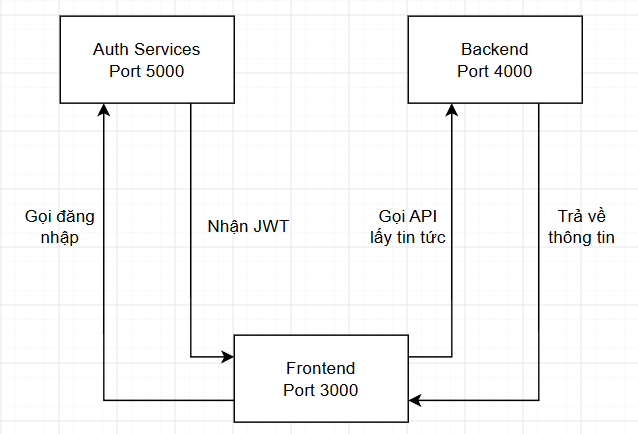
\includegraphics[width=0.75\linewidth]{Structure.png}\\[4pt]
  {\small\itshape (Khái niệm JWT — token đăng nhập — được giải thích ở cuối tài liệu.)}
\end{center}

Sinh viên không bắt buộc phải đọc hiểu chi tiết mã nguồn bên trong từng service — chỉ cần nắm vai trò và cách chúng giao tiếp như trên là đủ để triển khai.

\section{Mốc 0 — Chạy ứng dụng không cần Docker}

\begin{checklist}
  \item Chạy được backend bằng Node.js thuần.
  \item Chạy/build được frontend bằng Node.js thuần.
  \item Cho frontend gọi được sang backend, xác nhận dữ liệu hiển thị đúng.
\end{checklist}

\section{Mốc 1 — Đưa mã nguồn lên GitHub}

\begin{checklist}
  \item Tạo repo chung, cấu trúc thư mục rõ ràng, \texttt{.gitignore} hợp lý.
  \item Đưa mã nguồn lên qua Pull Request, chia commit theo từng phần việc.
  \item Review và duyệt Pull Request trước khi merge vào nhánh chính.
\end{checklist}

\section{Mốc 2 — Đóng gói bằng Docker}

\begin{checklist}
  \item Viết Dockerfile riêng cho từng service, build và chạy thử độc lập.
  \item Viết \texttt{docker-compose.yml} chạy đồng thời cả ba service.
  \item Xác nhận ba service giao tiếp được với nhau khi chạy bằng Docker.
\end{checklist}

\section{Mốc 3 — Triển khai trên Windows}

\begin{checklist}
  \item Chạy được toàn bộ ứng dụng bằng Docker trên môi trường Windows.
\end{checklist}

\section{Mốc 4 — Triển khai trên Linux}

\begin{checklist}
  \item Chạy được toàn bộ ứng dụng bằng Docker trên môi trường Linux (máy ảo hoặc WSL2).
  \item Đối chiếu kết quả với Mốc 3, ghi nhận khác biệt (nếu có).
\end{checklist}

\section{Mốc 5 (tùy chọn) — Triển khai online có tên miền thật}

\begin{checklist}
  \item Kiếm một VPS (free hoặc thuê), triển khai ứng dụng lên đó.
  \item Kiếm một tên miền (mua hoặc miễn phí) và trỏ về VPS.
  \item Kiểm tra truy cập ứng dụng qua tên miền thật từ bên ngoài VPS.
  \item Giữ VPS hoạt động ổn định cho đến buổi bảo vệ.
\end{checklist}

\section{Báo cáo nộp kèm}

Tất cả minh chứng của các mốc trên (ảnh chụp terminal, trình duyệt, cấu hình, bản ghi tên miền...) tổng hợp vào một báo cáo duy nhất, gồm:

\begin{checklist}
  \item Thông tin chung: thành viên nhóm, link repo, link demo online.
  \item Mô tả kiến trúc hệ thống và cách ba service giao tiếp.
  \item Minh chứng thực hiện cho từng mốc từ Mốc 0 đến Mốc 4, và Mốc 5 nếu nhóm có thực hiện.
  \item Khó khăn gặp phải trong quá trình triển khai và cách khắc phục.
\end{checklist}

\section{Bảo vệ bài tập lớn}

Đến buổi bảo vệ, nhóm \textbf{demo lại trực tiếp} ứng dụng đang chạy (kèm bản online qua tên miền thật nếu có làm Mốc 5) và trả lời câu hỏi của giảng viên về các bước đã thực hiện. Điểm số ưu tiên tính trên kết quả chạy thực tế tại thời điểm bảo vệ, không chỉ dựa vào ảnh chụp trong báo cáo.

\section{Phổ điểm (tóm tắt)}

Thang điểm tổng \textbf{10 điểm}, chia theo các mốc ở trên; cộng thêm tối đa \textbf{+2.0} điểm nâng cao (CI/CD, reverse proxy/HTTPS, giám sát/logging), chặn trần ở 10.0. Mốc 5 là tùy chọn — không làm mốc này, nhóm vẫn có thể đạt tối đa 10.0 nếu hoàn thành tốt phần điểm nâng cao. Chi tiết tiêu chí trừ điểm xem tại tài liệu hướng dẫn triển khai.

\begin{longtable}{@{}p{9cm} p{2cm}@{}}
\toprule
\textbf{Phần} & \textbf{Điểm} \\
\midrule
\endhead
Mốc 0 — Chạy không cần Docker & 1.0 \\
Mốc 1 — GitHub & 1.0 \\
Mốc 2 — Dockerfile \& Compose & 1.0 \\
Mốc 3 — Windows & 1.0 \\
Mốc 4 — Linux & 1.0 \\
Báo cáo & 2.0 \\
Bảo vệ & 3.0 \\
\addlinespace
\textit{Mốc 5 (tùy chọn) — VPS \& domain} & \textit{+1.0} \\
\textit{Điểm cộng (CI/CD, reverse proxy/HTTPS, giám sát)} & \textit{+2.0} \\
\bottomrule
\end{longtable}

\section*{JWT (token đăng nhập) là gì?}

JWT (JSON Web Token) là một \textbf{chuỗi ký tự} do \texttt{auth-service} tạo ra sau khi kiểm tra mật khẩu đúng, đóng vai trò như một "thẻ ra vào" tạm thời cho quản trị viên — tương tự vé xem phim: mua vé (đăng nhập) một lần, sau đó chỉ cần đưa vé (token) ra là được vào mà không cần trình chứng minh nhân dân lại từ đầu.

\begin{itemize}[itemsep=3pt]
  \item Sau khi đăng nhập thành công, \texttt{frontend} lưu token này lại (trong trình duyệt) và đính kèm vào mọi yêu cầu thêm/sửa/xóa tin tức gửi tới \texttt{backend}.
  \item \texttt{backend} không cần hỏi lại \texttt{auth-service} xem token có hợp lệ không — vì hai service này được cấu hình dùng chung một \textbf{khóa bí mật} (\texttt{JWT\_SECRET}), giống như hai bên cùng giữ một con dấu giống hệt nhau: bên nào cũng có thể tự kiểm tra chữ ký trên "vé" mà không cần gọi điện hỏi bên kia.
  \item Token có \textbf{thời hạn} (ví dụ 2 giờ) — hết hạn thì phải đăng nhập lại để lấy token mới.
\end{itemize}

Về mặt triển khai, sinh viên chỉ cần nhớ một điều: \textbf{giá trị \texttt{JWT\_SECRET} cấu hình cho \texttt{backend} và \texttt{auth-service} phải giống hệt nhau}, nếu không hai service sẽ "không hiểu" token của nhau và mọi thao tác quản trị sẽ báo lỗi.

\end{document}
